\section{System identification}
\label{cap:system_identification}

A test flight needed to be made, in order to identify parameters $P_1 \hdots P_6$, introduced in chapter \ref{chap:uav_dynamics}. Several methods exist for system identification for both time and frequency domain. Despite theirs advantages, one have to excite system poles and zeros in a way that could lead to damage of the system and its surroundings. In case of highly unstable UAV, testing by a step response or frequency response is mostly unwanted. Instead of that the model can be fitted to arbitrary data using a mathematical optimization approach. The test flight, which was conducted by a human operator, consisted mainly of hovering above one place with small oscillations in all axis. All data used for following identification were gathered from the onboard \emph{px4flow} optical flow sensor (including ultrasonic rangefinder). The data were received and logged in constant rate and coupled with appropriate control action of the operator. Since all searched parameters are part of the first order system eq. (\ref{eq:first_order_stab}), we can write down its discrete differential equation

\begin{equation}
q_{[n]} = P_Aq_{[n-1]} + P_Bu_{[n-1]},
\end{equation}
\\
where $P_A$, $P_B$ are unknown constants of the transfer function. If supposing that, all sensors are perfect and there are no other effects on the system, this equation should hold for all measured samples. When considering all samples, the set of equations can be written in a matrix form as follows:

\begin{equation}
\textbf{b} = \textbf{A}\textbf{p},
\label{eq:bap}
\end{equation}
\\
where $\textbf{A} \in \mathbb{R}^{(m-1)\times2}$ represents matrix of the set of equations, $\textbf{b} \in \mathbb{R}^{(m-1)}$ is the left-hand side of the equation, $\textbf{p} \in \mathbb{R}^{2}$ is the vector of parameters we are looking for, and $m$ being the number of samples. Parameters \textbf{b}, \textbf{A}, \textbf{p} are created as follows:

\begin{equation}
\textbf{A} = \begin{bmatrix}
q_{[1]} & u_{[1]} \\
q_{[2]} & u_{[2]} \\
\vdots & \vdots \\
q_{[m-1]} & u_{[m-1]} \\
\end{bmatrix},
\textbf{b} = \begin{bmatrix}
q_{[2]} \\
q_{[3]} \\
\vdots\\
q_{[m]}
\end{bmatrix},
\textbf{p} = \begin{bmatrix}
P_A \\
P_B
\end{bmatrix}.
\end{equation}

Due to the fact that the system description does not cover all phenomena and the measured data is noisy, the equation (\ref{eq:bap}) does not necessary hold. But we can still estimate \textbf{p} in a way that $\norm{\textbf{Ap-b}}_2^2$ is minimal. Thus the supplied set of equations needs to be overdetermined to provide sufficient accuracy of estimated parameters. The solution is then optimal in terms of least squares of \textbf{r}, where $\textbf{r} = \textbf{Ap-b}$ is a vector of residuals of the equation system. This optimization problem can be solved e.g. by using operator '\textit{\textbackslash}' in Matlab.

\subsection{Attitude subsystem identification}
\label{cap:attitude_subsystem_identification}

Four parameters, $P_1$, $P_2$ for \texttt{x} axis and $P_3$, $P_4$ for \texttt{y} axis, need to by identified. Assuming the system is decoupled and the low-level stabilization drives both subsystems identically\footnote{Further experiments show that both axis can be driven by the same controller utilizing a single model.}, we can identify a model using only one of them. Following experiment was conducted using a manually controlled UAV equipped with the \textit{px4flow} optical flow sensor. Data from the experiment (fig. \ref{fig:iden1}) are both unfiltered and captured onboard using a dedicated logging device. Unit of measurement of the input signal represents a difference from a mean PPM\footnote{Pulse Position Modulation is a common communication protocol used on unmanned vehicles.} signal pulse length, measured using a hardware timer. They are directly proportional to the desired attitude angle of the UAV.

\begin{figure}[h]
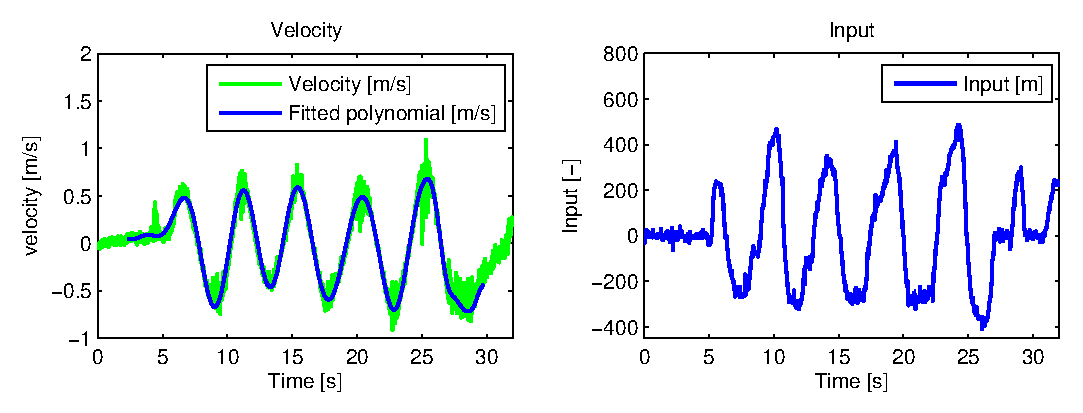
\includegraphics[width=1\textwidth]{fig/iden1.eps} 
\caption{Identification data - attitude.}
\label{fig:iden1}
\end{figure}

The speed signal has to be differentiated to identify the first order transfer function from the input to the acceleration. Discrete differentiation of the signal was found impractical, due to its large noise component. But when fitting a smooth function to the data, the derivative can be computed analytically. The polynomial function was chosen to fit the data since it can be easily differentiated and it can be found easily. Using the approach described above, constants $P_1$ and $P_2$ were obtained as:

\begin{equation}
P_1 = 0.9799, P_2 = 5.0719 \times 10^{-5}.
\label{eq:constants1}
\end{equation}

Having these constants, the attitude system can be completed from eq. (\ref{eq:attitude_LTI}) with particular values:

\begin{equation}
\begin{split}
\mathbf{A}_{x, y} = \begin{bmatrix}
1 & 0.0114 & 0 \\
0 & 1 & 0.0114 \\
0 & 0 & 0.9799
\end{bmatrix}, \mathbf{B}_{x, y} = \begin{bmatrix}
0\\
0\\
5.0719 \times 10^{-5}
\end{bmatrix}.
\end{split}
\label{eq:attitude_LTI_identified}
\end{equation}

The system can be further tested by estimating all states in open-loop from the measured input. We can evaluate its performance empirically by comparing estimates with measured data.

\begin{figure}[h]
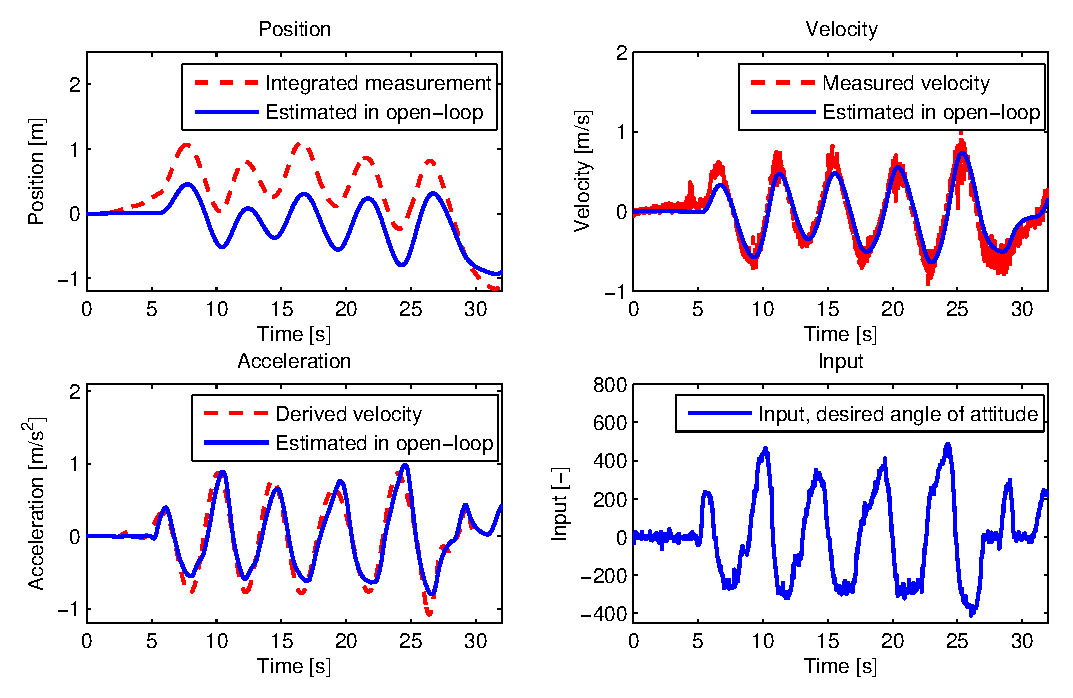
\includegraphics[width=1\textwidth]{fig/iden2.eps} 
\caption{Identification - open loop estimation of attitude system states}
\label{fig:iden2}
\end{figure}

As it can be seen in fig. \ref{fig:iden2}, states estimated in open-loop are tracking the genuine values without a significant error. Some drift can be seen in the position, after the second integrator. But the model fits the measured data sufficiently, at least for purpose of the control design. 

\subsection{Altitude subsystem identification}

For the purpose of altitude identification, another flight was realized. Again, with an intention to excite the system's dynamics. In this case, the measured state is an altitude. It is supplied by an ultrasonic rangefinder which works in a range from $0.3$\jed{m} to $4$\jed{m}. The sensor is implemented on the \emph{px4flow} unit and although the data is sent together with the optical flow, its actual rate is about $20$\jed{Hz}. Data were again fitted with polynomial and further differentiated into other states. Figure \ref{fig:iden3} shows data on which parameters $P_5$, $P_6$ were found. In this particular situation, input signal had to be shifted to cancel the DC\footnote{Supposing the force caused by the gravity of Earth is a constant, the total thrust signal contains a DC component countering the gravitational pull.} component which countered the gravitational acceleration. The input offset was found by another optimization with a cost computed as a sum of sums of quadratic errors of all state open-loop estimations.

\begin{figure}[h]
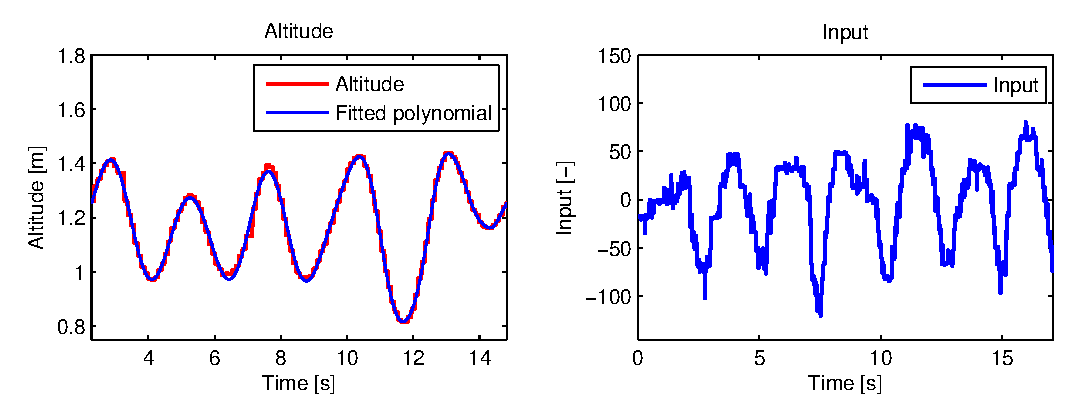
\includegraphics[width=1\textwidth]{fig/iden3.eps} 
\caption{Identification data - altitude}
\label{fig:iden3}
\end{figure}

The measurement unit of the input signal is again a time difference from a mean PPM pulse measured in discrete steps of a hardware timer. Following parameters were found using the \emph{least squares method} described in the beginning of this chapter:

\begin{equation}
P_5 = 0.9519, P_6 = 0.0012 \times 10^{-5}.
\label{eq:constants2}
\end{equation}

Having these constants, the attitude system can be completed from eq. (\ref{eq:altitude_LTI}) with the particular values

\begin{equation}
\begin{split}
\mathbf{A}_{z} = \begin{bmatrix}
1 & 0.0114 & 0 & 0\\
0 & 1 & 0.0114 & 0\\
0 & 0 & 0 & 1 \\
0 & 0 & 0 & 0.9519
\end{bmatrix}, \mathbf{B}_{z} = \begin{bmatrix}
0 & 0\\
0 & 0\\
0 & -g\\
0.0012 & 0
\end{bmatrix},
\end{split}
\label{eq:altitude_LTI_with_constants}
\end{equation}
\\
where $g \approx 9.8 ms^{-2}$ is the gravitational acceleration.

As can be seen in fig. \ref{fig:iden4} the open-loop estimation holds fairly up to the speed state. The altitude drifts heavily in a horizon of seconds, which indicates that the LTI system is not identified as good as in case of the attitude system. It could be due to omitting some physical phenomena e.g. in case of the rotor thrust or because of the linearization itself.

\subsection{Yaw subsystem identification}

The system could be identified by exactly the same procedure as the previous subsystems. But in our case, the UAV is not equipped with any device to measure its yaw angle or rate. It is stabilized by dead-reckoning from IMU\footnote{Inertial Measurement Unit - measures accelerations and rotational speeds of the UAV.} (yaw rate measured by a gyro). The actual data from IMU are present only in integrated stabilization and are not sent to the custom control board. This would require a modification of the used stabilization board.

\begin{figure}[h]
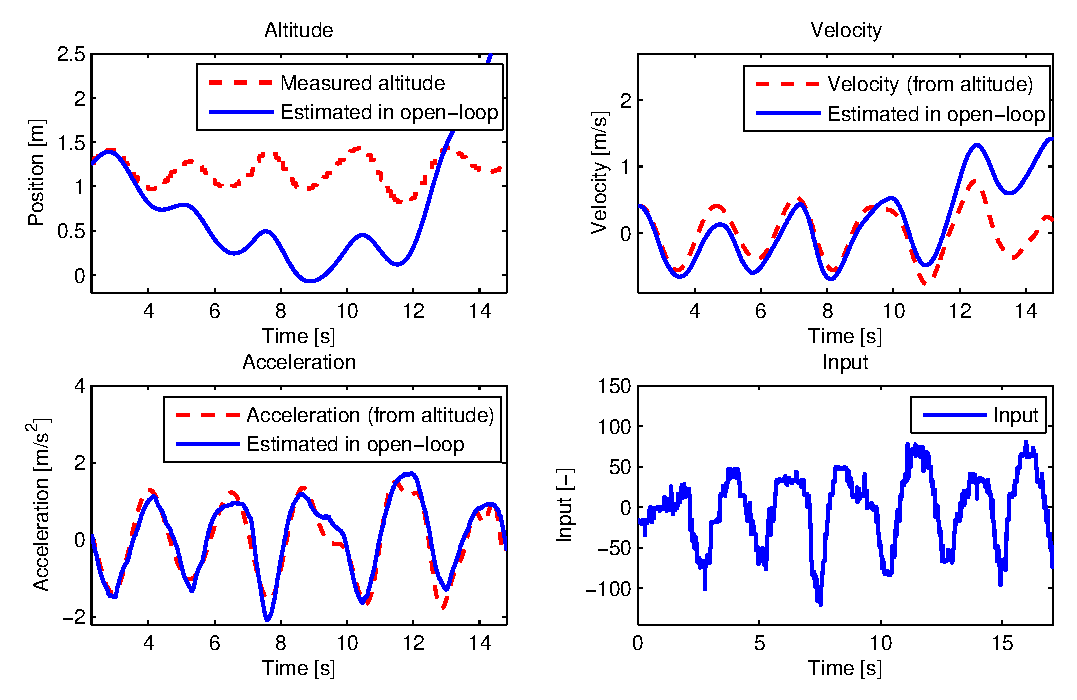
\includegraphics[width=0.99\textwidth]{fig/iden4.eps} 
\caption{Identification - open loop estimation of altitude system states.}
\label{fig:iden4}
\end{figure}

\subsection{Summary}

This chapter discussed the identification of parameters of the dynamical model presented in chapter \ref{chap:uav_dynamics}. Mathematical optimization was used to fit a model to measured data in terms of least squares of residuals. We were able to find common parameters for both axis of the attitude model $P_1$, $P_2$, and parameters of the altitude model $P_3$, $P_4$. Using this information state space representation of both systems was constructed. It can be further used for state estimation and system control as it is shown in following chapters. The identification is considered successful by means of open-loop estimation error as it can be seen in presented figures. The absence of the yaw measurement could be solved by adding e.g. a magnetometer or an additional camera system.